% !TEX root = calculus.tex


\chapter{DERIVATIVE}
\label{derivative}

\athr The previous dialogue gave us an opportunity to introduce the concept of a \emph{derivative} for a specific example from physics (the instantaneous velocity of a body moving non-uniformly along a straight line). Now let us examine this concept from a purely mathematical viewpoint without assigning any physical meaning to the mathematical symbols used.

\begin{figure}[!ht]%[13]{r}{0.5\textwidth}
\centering
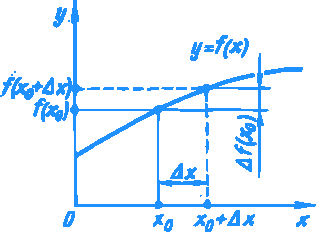
\includegraphics[width=0.6\textwidth]{figures/fig-36.pdf}
\caption{Examining concept of a derivative on an arbitrary function.}
\label{fig-36}
\end{figure}

\fig{fig-36} shows a graph of an arbitrary function $y = f (x)$. Let us select an arbitrary point $x= x_{0}$ from the domain of the function. In the subsequent argument this point is considered as \emph{fixed}. Now consider another point $x$ from the domain of the function and introduce a notation $\Delta x = x -	x_{0}$. The value $\Delta x$ is called the \emph{increment of the independent variable}. The increment is considered with respect to the fixed point $x_{0}$. Depending on the point $x$, the value of $\Delta x$ may. be larger or smaller, positive or negative.

Now let us examine a difference between the values of the function at points $x = x_{0} + \Delta x$ and $x = x_{0}$:
\begin{equation*}%
\Delta f (x_{0}) = f (x_{0} + \Delta x) - f(x_{0})
\end{equation*}
The difference  $\Delta f (x_{0})$ is said to be the \emph{increment of a function $f$ at a point $x_{0}$}. Since $x_{0}$ is fixed, $\Delta f (x_{0})$ should be considered as a function of a variable increment $\Delta x$ of the independent variable.

\rdr Then it is probably more logical to denote this function by $\Delta f (\Delta x)$, and not by $\Delta f (x_{0})$, isn't it?

\athr Probably, you are right. However, the accepted notation is $\Delta f (x_{0})$. Such a notation emphasized the fact that the increment of $f$ (in other words, the given function of $\Delta x$ is referred to point $x_{0}$.

With the concepts of the increment introduced, it is not difficult to evaluate the rate of change of $f$ close to $x_{0}$.


\rdr This rate should be described by the ratio $\dfrac{\Delta f(x_{0})}{\Delta x}$. For instance, if we compare $\Delta f(x_{0})$ with an increment of t at another point from the domain of the function (say, point $x = x_{1}$), we may obtain an inequality
\begin{equation*}%
\frac{\Delta f (x_{1})}{\Delta x} > \frac{\Delta f (x_{0})}{\Delta x} 
\end{equation*}
and therefore conclude that the rate of change of $f$ close to point $x_{1}$ is greater than that close to $x_{0}$.

\athr Please, be careful. You have not said anything about the vague increment $\Delta x$. If $\Delta x$ is too large, the inequality you have just mentioned may lead to a wrong conclusion. I shall make myself clearer by referring to
\fig{fig-37}. As you see,
\begin{equation*}%
\frac{\Delta f (x_{1})}{\Delta x} > \frac{\Delta f (x_{0})}{\Delta x} 
\end{equation*}
You must agree, however, that close to point $x_{0}$ the function changes much faster (the graph of the function has a steeper slope) than in the vicinity of $x_{1}$.

\begin{figure}[!ht]%[13]{r}{0.5\textwidth}
\centering
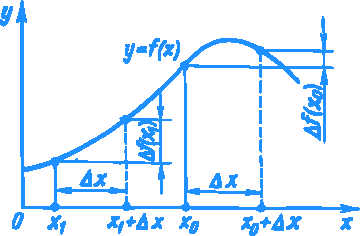
\includegraphics[width=0.6\textwidth]{figures/fig-37.pdf}
\caption{Examining concept of a derivative on an arbitrary function.}
\label{fig-37}
\end{figure}

\rdr It is necessary that the value of the increment $\Delta x$  be sufficiently small. The smaller is $\Delta x$ the more accurate is the information about the rate of change of the function close to the point under consideration.

\athr Well, we can do even better than this. We may, for example, consider the limit of the ratio $ \dfrac{\Delta f (x_{0})}{\Delta x} $ for $\Delta x \to 0$	(remember	the	previous dialogue). 

\rdr This limit will characterize the \emph{rate of change} of the function $f$ directly at $x =x_{0}$. 

\athr Exactly. Let us calculate the limit in detail:
\begin{equation}%
\lim\limits_{\Delta x \to 0}  \frac{\Delta f (x_{0})}{\Delta x} = \lim\limits_{\Delta x \to 0}   \frac{\Delta f (x+ x_{0}) - f (x_{0}) }{\Delta x}
% eq 1 of 09
\label{limit-in-detail}
\end{equation}
and examine first of all the mathematical nature of this limit.

\rdr Since point $x_{0}$ is fixed, it is evidently the limit of the ratio of two functions of  $\Delta x$  for  $\Delta x \to 0$ .

\athr Let us denote these functions by $F$ and $G$:
\begin{equation*}%
 F(\Delta x) = f( x_{0}+ \Delta x) - f(x_{0}),	\qquad G (\Delta x) = \Delta x
\end{equation*}


\rdr Limit \eqref{limit-in-detail} is then 
\begin{equation*}%
\lim\limits_{\Delta x \to 0} \frac{ F(\Delta x) }{ G(\Delta x) }
\end{equation*}
where $\lim\limits_{\Delta x \to 0}  F(\Delta x)=0$ and $\lim\limits_{\Delta x \to 0}  G(\Delta x)=0$. Hence, we have here a limit similar to that discussed at the end of Dialogue Seven, namely, a limit of the type $\dfrac{\infty}{\infty}$. 

\athr Right. This limit, that is, the limit of the type $\dfrac{\infty}{\infty}$ the main subject of this dialogue.

The primary requirement in this case is the \emph{existence} of the limit. It means that the function $f$ should be such that
\begin{equation*}%
\lim\limits_{\Delta x \to 0}F (\Delta x) = 0
\end{equation*}
The necessary condition for satisfying this equality is the \emph{continuity} of $f$ at $x =x_{0}$ But we shall discuss this problem later.


If the limit of the type  $ \dfrac{\infty}{\infty}$ (in other words, limit \eqref{limit-in-detail}) does exist, it is called ``the derivative of the function $f$ at point $x = x_{0}$ and usually denoted by $f'(x_{0})$.''

\begin{mytheo}{Definition}
The derivative of a function $f$ at a point $x_{0}$ (denoted by $f'(x_{0})$) is the limit of the ratio of an increment of the function $f$ at the point $x_{0}$ (denoted by  $\Delta f(x_{0})$) to an increment $\Delta x$ the independent variable for $\Delta x \to 0$:
\begin{equation*}%
f'(x_{0}) = \lim\limits_{\Delta x \to 0} \frac{\Delta f(x_{0})}{\Delta x}
\end{equation*}
or, in a more detailed notation,
\begin{equation}%
f'(x_{0}) = \lim\limits_{\Delta x \to 0} \frac{\Delta f(x_{0})}{\Delta x}
% eq 2 of 9
\label{derivative-defn}
\end{equation}
\end{mytheo}
Note that you are already familiar with the right-hand side of equation \eqref{derivative-defn} (cf. expression \eqref{instant-velocity} from the previous dialogue).

\rdr Actually the derivative of the function $f$ at point 0 is the limit of the function 
\begin{equation*}%
\frac{F}{G} =	\frac{ f (x_{0} + \Delta x) - f (x_{0})}{\Delta x}
\end{equation*}
at $ \Delta x = 0$. The independent variable of the function $\dfrac{F}{G}$
is the increment $\Delta x$. 

\athr You are quite right. However, in what follows you must use the definition of the derivative as formulated above. This definition does not involve the function $\dfrac{F}{G}$ of $\Delta x$ since this function plays, as you understand, only an auxiliary role. We should simply bear in mind that the phrase ``the limit of the ratio of an increment $\Delta f (x_{0})$ to an increment $\Delta x$ for $\Delta x \to 0$'' describes the limit of a function of $\Delta x$, i.e. the function $\dfrac{F}{G}$, which is considered at $\Delta x = 0$.

The derivative can be also interpreted \emph{in terms of geometry}.

\rdr Shall we do it by using again the tangent to the graph of a function?

\athr Yes, of course. Let us take the graph $y = f (x)$ (\fig{fig-38}), fixing a point $x = x_{0}$. Consider an increment $\Delta x_{1}$  of the argument; the corresponding increment of the function at point $ x_{0}$ is $\Delta f_{1} (x_{0})$. Denote the slope of the chord $AB_{1}$ by $\alpha_{1}$ it is readily apparent that 
\begin{equation*}%
\frac{\Delta f_{1}(x_{0})}{\Delta x_{1}}  = \tan \alpha_{1}
\end{equation*}

\begin{figure}[!ht]%[13]{r}{0.5\textwidth}
\centering
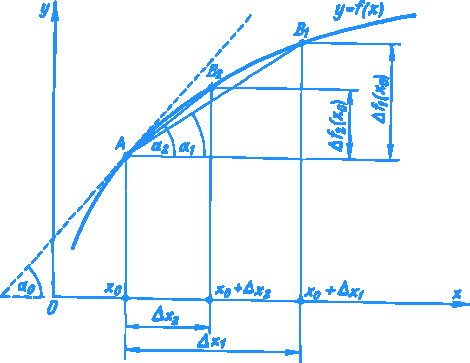
\includegraphics[width=0.8\textwidth]{figures/fig-38.pdf}
\caption{Examining concept of a derivative geometrically.}
\label{fig-38}
\end{figure}

Next take an increment $\Delta x_{1}$ (so that $\Delta x_{2}< \Delta x_{1}$). This increment corresponds to the increment $f_{2}(x_{0})$ of the function $f$ at point $x_{0}$. Denote the slope of the chord $AB_{2}$ by $\alpha_{2}$; it is similarly quite apparent that 
\begin{equation*}%
\frac{\Delta f_{2}(x_{0})}{\Delta x_{2}}  = \tan \alpha_{2}
\end{equation*}


Further, take an increment $\Delta x_{3}$ (so that $\Delta x_{3}< \Delta x_{2}$), and so on. As a result, we obtain an infinitesimal sequence of increments of the independent variable:
\begin{equation*}%
\Delta x_{1}, \, \Delta x_{2},  \,  \Delta x_{3},  \, \Delta x_{4},  \, \ldots \Delta x_{n},  \, \ldots
\end{equation*}
and the corresponding infinitesimal sequence of increments of the function at point $x_{0}$: 
\begin{equation*}%
\Delta f_{1} (x_{0}),  \, \Delta f_{2} (x_{0}),  \, \Delta f_{3} (x_{0}),  \, \Delta f_{4} (x_{0}),  \, \ldots \Delta f_{n} (x_{0}),  \, \ldots
\end{equation*}
This leads to a new sequence of the values of the tangent of the slopes of the chords $AB_{1}, AB_{2}, AB_{3}, \ldots AB_{n}, \ldots$. obtained as a sequence of the ratios of the two sequences given above
\begin{equation}%
\tan \alpha_{1},  \, \tan \alpha_{2},  \, \tan \alpha_{3},  \, \tan \alpha_{4},  \, \dots \tan \alpha_{n},   \, \ldots 
% eq 3 sec 9
\label{geom-defn-derivative}
\end{equation}
Both sequences $\Delta x_{n}$ and $\Delta f_{n} (x_{0})$ converge to zero. And what can be said about the convergence of the sequence ($\tan \alpha_{n}$) or, in other words, the sequence $\dfrac{\Delta f_{n} (x_{0})}{\Delta x_{n}}$?

\rdr Obviously, the sequence $\dfrac{\Delta f_{n} (x_{0})}{\Delta x_{n}}$ converges to $f' (x_{0})$. In other words, the limit of  $\dfrac{\Delta f_{n} (x_{0})}{\Delta x_{n}}$ is the derivative of $f$ at $x_{0}$. 

\athr What are the grounds for this conclusion? 

\rdr Why, isn't it self-evident? 

\athr Let me help you. Your conclusion is based
on \emph{Definition 2} of the limit of function at a point. Don't you think so?

\rdr Yes, I agree. Indeed, a certain number (in this case $f' (x_{0}$ is the limit of a function $\Phi (\Delta x)$ (in this case $\Phi = \dfrac{F}{G}$) at $\Delta x = 0$ if for any sequence $\Delta x_{n}$ convergent to zero the corresponding sequence $(\Phi (\Delta x_{n}))$ converges to this number. Sequence \eqref{geom-defn-derivative} is precisely the sequence $(\Phi (\Delta x_{n}))$ in our case.

\athr Correct. We have thus found that $\lim\limits_{n \to \infty} \tan \alpha_{n} = f' (x_{0})$. Now look at \fig{fig-38} and tell me which direction is the limit for the sequence composed of the chords  $AB_{1}, \, AB_{2}, \,  AB_{3},  \, \ldots AB_{n},  \, \ldots$? 

\rdr It is the direction of the \emph{tangent} to the graph $f (x)$ at point $x = x_{0}$.

\athr Correct. Denote the slope of the tangent line by $\alpha_{0}$. Thus
\begin{equation*}%
\lim\limits_{n \to \infty} \tan \alpha_{n} = \tan \alpha_{0}
\end{equation*}
Consequently,
\begin{equation*}%
f' (x_{0}) = \tan \alpha_{0}
\end{equation*}
We thus obtain the following geometrical interpretation of the derivative:
\begin{mytheo}{}
The derivative of a function $f$ at a point $x_{0}$ is defined by the slope of the tangent to the graph of the function $f$ at the point $x = x_{0}$.
\end{mytheo}

Note that the slope of the tangent is measured relative to the positive direction of the abscissa axis, so that the derivative of $f$ at point $x_{0}$ in \fig{fig-39} is positive (at this point $\tan \alpha_{0} > 0$), while at point $x_{0}$ the derivative of $f$ is negative $\tan \alpha_{0} < 0$).

\begin{figure}[!ht]%[13]{r}{0.5\textwidth}
\centering
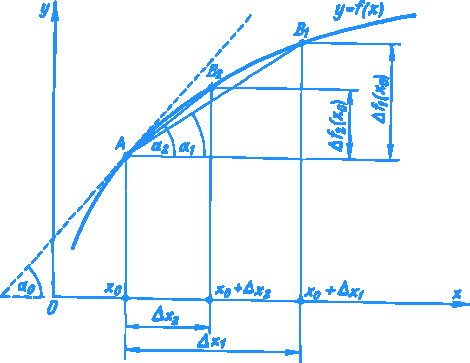
\includegraphics[width=0.8\textwidth]{figures/fig-38.pdf}
\caption{Examining concept of a derivative geometrically.}
\label{fig-39}
\end{figure}

But the geometrical interpretation of the derivative must not upstage the basic idea that
\begin{mytheo}{}
The derivative of a function $f$ at a point $x_{0}$ is the rate of change of $f$ at this point.
\end{mytheo}

In the previous dialogue we analyzed the function $s (t)$ describing the dependence of the distance covered by a body during the time $t$. In this case the derivative of $s (t)$ at a point $t = t_{0}$ is the \emph{velocity} of the body at the moment of time $t = t_{0}$. If, however, we take $v (t)$ as the initial function (the instantaneous velocity of a body as a function of time), the derivative at  $t = t_{0}$ will have the meaning of the acceleration of the body at  $t = t_{0}$. Indeed, \emph{acceleration} is the \emph{rate of change of the velocity} of a body.

\rdr Relation \eqref{derivative-defn} seems to allow a very descriptive (if somewhat simplified) interpretation of the derivative. We may say that
\begin{mytheo}{}
The derivative of a function $y = f (x)$ at a point $x = x_{0}$ shows how much steeper the change in $y$ is in comparison with the change in $x$ in the neighbourhood of $x = x_{0}$.
\end{mytheo}

\athr This interpretation of the derivative is quite justified, and it may be useful at times.

Getting back to the geometrical interpretation of the derivative, we should note that it immediately leads to the following rather important

\begin{mytheo}{Conclusions:}
\begin{enumerate}[label=\textsection]
\item The derivative of a function $f = \text{const}$ (the derivative of a constant) is zero at all the points.
\item The derivative of a junction $f = ax + b$ (where $a$ and $b$ are constants) is constant at all the points and equals $a$.
\item The derivative of a function $f = \sin x$ is zero at the points $x = + \pi n$ (at these points the tangent to the graph of the function is horizontal).
\end{enumerate}
\end{mytheo}

This ``list'' could, of course, be expanded.

Next I would like to attract your attention to the following: from the viewpoint of mathematics a derivative of a function must also be considered as a certain function.

\rdr But the derivative is a limit and, consequently, a \emph{number}!

\athr Let us clarify this. We have fixed a point $x = x_{0}$ and obtained for a function $f (x)$ at this point the number
\begin{equation*}%
\lim\limits_{\Delta x \to 0} \frac{\Delta f (x_{0})}{\Delta x}
\end{equation*}
For each point $x$ (from the domain of $f$) we have, in the general case, its own number
\begin{equation*}%
\lim\limits_{\Delta x \to 0} \frac{\Delta f (x)}{\Delta x}
\end{equation*}
\begin{mytheo}{}
This gives a mapping of a certain set of numbers $x$ onto a different set of numbers $\lim\limits_{\Delta x \to 0} \dfrac{\Delta f (x)}{\Delta x}$. The function which represents this mapping of one numerical set onto another is said to be the derivative and is denoted by $f'(x)$.
\end{mytheo}

\rdr I see. So far we have considered only one value of the function $f (x)$, namely, its value at the point $x = x_{0}$.

\athr I would like to remind you that in the previous dialogue we analyzed $v (t) $ which was the derivative of $s (t)$. The graphs of the two functions (i.e. the initial function $s (t)$ and its derivative $v (t)$) were even compared in \fig{fig-35}.

\rdr Now it is clear.

\athr I would like to make two remarks with regard to $f' (x)$.

\textcolor{IndianRed}{\textbf Note 1}. A function $f' (x)$ is obtained only by using a function  $f (x)$. Indeed,
\begin{equation}%
\boxed{
f' (x) = \lim\limits_{\Delta x \to 0} \frac{f (x + \Delta x) - f(x)}{\Delta x}}
\label{note-1-def}
%eq-4 of 9
\end{equation}
It is as if there is a certain operator (recall \hyperref[function]{Dialogue Four}) which generates $f' (x)$ at the output in response to $f (x)$ at the input. In other words, this operator, applied to the function $f (x)$, ``generates'' $f' (x)$. This operator is usually
denoted by $\dfrac{d}{dx}$. This notation should be interpreted as a single entity and not as a ratio (it reads: ``$d$ over $dx$''). 

Consider an ``image''
\begin{equation*}%
\frac{d}{dx} \boxed{1} = \boxed{2}. 
\end{equation*}
The squares in this
expression symbolize the familiar ``windows''. ``Window'' 1 is to input $f (x)$, while ``window'' 2 outputs $f' (x)$. Thus,
\begin{equation}%
\boxed{
\frac{d}{dx}  f (x) = f' (x)}
\label{note-1-def2}
%eq-5 of 9
\end{equation}

\begin{mytheo}{Definition:}
The operation of obtaining $f' (x)$ from $f (x)$ is said to be the differentiation of $f (x)$.
\end{mytheo}
The operator $\dfrac{d}{dx}$ performs this operation over $f (x)$ and is said to be the operator of differentiation.

\rdr But what exactly is $\dfrac{d}{dx}$ doing with $f (x)$? 

\athr It is exactly the operation prescribed by \eqref{note-1-def}.
We may say that $\dfrac{d}{dx}$ ``constructs'' the ratio 
\begin{equation*}%
\frac{(x + \Delta x) - f(x)}{ \Delta x}
\end{equation*}
from $f (x)$ and determines the limit of this ratio (regarded as a function of $\Delta x$) at $dx = 0$.

\rdr In other words, the operator $dx$ performs  a certain limit transition operation, doesn't it? 

\athr Certainly. The whole	differential	calculus (and with it, integral calculus) can be formulated in terms of certain limit transitions. 

\rdr Why should we introduce an operator $\dfrac{d}{dx}$ if it represents nothing else but the limit transition operation described by \eqref{note-1-def}?

\athr You have posed a very important question. The problem is that if we had formulated differential calculus in terms of limits, using the relations of type \eqref{note-1-def}, all books on calculus should have been increased in their volume several-fold and become hardly readable. The use of the relations of type \eqref{note-1-def2}, instead of \eqref{note-1-def}, makes it possible to avoid this.

\rdr But how can we use the relations of type \eqref{note-1-def2} \emph{without implicitly applying} the relations of type \eqref{note-1-def}?

\athr What is done is this. 

First, using \eqref{note-1-def}, we find the result of applying the operator $\dfrac{d}{dx}$ to a sum, product, and ratio of functions, and to composite
or inverse functions \emph{provided} that the result of applying the operator to the initial function (or functions) is \emph{known}. In other words, the first step is to establish the \emph{rules for the differentiation of functions}.

Second, using  \eqref{note-1-def}, we find out the result of applying $\dfrac{d}{dx}$ to some basic elementary functions (for instance, $y = x^{n}, \, y = \sin x, \,\, \text{and} \,\, y = \log x$).

After these two steps are completed you can practically forget about the relations of type \eqref{note-1-def}. \emph{In order to differentiate a function, it is sufficient to express the function via basic elementary functions (the derivatives of which were obtained earlier) and apply the rules for differentiation.}

\rdr Does it mean that the relations of type \eqref{note-1-def}
could be put aside after they have been used, first, for compiling a \emph{set of differentiation rules} and, second, for making a \emph{table of derivatives for basic elementary functions}?

\athr Yes, this is the procedure. Using the differentiation rules and the table of derivatives for some basic elementary functions you are in a position to forget about the relations of type \eqref{note-1-def} and are free to proceed further by using the ``language'' of the relations of type \eqref{note-1-def2}. A formal course of differential calculus could skip the analysis of limit transition operations, that is, the relations of type \eqref{note-1-def}. It is quite sufficient for a student to learn a set of differentiation rules and a table of derivatives of some functions.

\rdr I certainly prefer to be given the foundation.

\athr Our next dialogue will be devoted to a discussion of the programme of actions as outlined above. At the first step of the programme, the main rules for differentiation will be established on the basis of the relations of \eqref{note-1-def} and, in addition, the derivatives of three functions $y = x^{2}, \, y = \sin x, \, \, \text{and} \,\, y = \log_{a} x$ will be obtained. At the second step, we shall obtain (without reference to the relations of type \eqref{note-1-def}) the derivatives of the following functions: 

$y=x^{n}, \, y=x^{-n}, \, y= \sqrt{x}, \, y= \cos x, \, y= \tan x, \, y = \cot x, \, y = \arcsin x, \, y = \arccos x,\,  y= \arctan x, y = \arccot x, \,\, \text{and} \,\, y = a^{x}$.

\rdr I'll be looking forward to the next dialogue. By the way, you wanted to make one more remark about the derivative $f' (x)$.

\athr \textcolor{IndianRed}{Note 2} concerns the natural domain of a derivative. Let a set $D$ be the domain of $f (x)$. The question is whether $D$ is also the domain of $f' (x)$.

\rdr In any case, the domain of $f' (x)$ cannot be wider than the domain of $f (x)$ because in order to find $f' (x)$ we use $f (x)$.

\athr A carefully balanced answer, to be sure. The domain of $f' (x)$ is in the general case a subset of $D$. It is obtained from $D$ as a result of elimination of those points $x$ for which $\lim\limits_{\Delta x \to 0} \dfrac{\Delta f (x)}{\Delta x}$ does not exist. By the way, this subset is called the \emph{domain of differentiability} of $f (x)$. 

\rdr What are the \emph{conditions of differentiability} of $f(x)$ at any specific point $x$?

\athr Obviously, these conditions are identical to those of the existence of $\lim\limits_{\Delta x \to 0} \dfrac{\Delta f (x)}{\Delta x}$ at point $x$. We have
already observed that it is the limit of the type {\smaller $\dfrac{\infty}{\infty}$}, which necessitates that both the numerator and denominator tend to zero. It means that $f (x)$ must be continuous at $x$. The following theorem could be proved rigorously.

\begin{mytheo}{Theorem:}
The continuity of a function $f (x)$ at a point $x$ is a necessary condition for the existence of $f' (x)$ at $x$.
\end{mytheo}
However, we shall not give the proof of this theorem here. The simple qualitative arguments given above will suffice.

\rdr I wonder whether the continuity of a function is also a \emph{sufficient} condition for its differentiability.

\athr No, it is not. Consider, for example, the function $y = | \log x |$. It is sufficient only to look at its graph (\fig{fig-40}) to conclude that at $x = 1$ the tangent to the graph of the function is, strictly speaking, nonexistent (on approaching $x = 1$ from the left we have one tangent, viz., the straight line $AA$, while on approaching $x = 1$ from the right we have another tangent, viz., the straight line $BB$). It means that $y = | \log x |$ does not have a derivative at $x = 1$, although the function is continuous at this point.

\begin{figure}[!ht]%[13]{r}{0.5\textwidth}
\centering
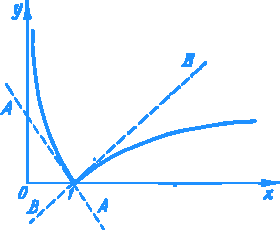
\includegraphics[width=0.6\textwidth]{figures/fig-40.pdf}
\caption{Examining the derivative of the function $y = | \log x |$.}
\label{fig-40}
\end{figure}


In conclusion, let us turn to one interesting property of differentiable functions. 

Let $f (x)$ be a differentiable function, and its increment $\Delta f$ at $x$ be related to the increment $\Delta x$ of the argument as follows:
\begin{equation}%
\Delta f= f' (x) dx +  \eta (\Delta x) \Delta x
\label{diff-func}
%6 of 9
\end{equation}
where $ \eta (\Delta x)$is a function of $ \Delta x$. 

By dividing both parts of \eqref{diff-func} by $\Delta x$, we obtain
\begin{equation*}%
\frac{\Delta f}{\Delta x} =f' (x) + \eta (\Delta x)
 \end{equation*}

Passing to a limit in both sides of the last equation for $\Delta x$ gives $\lim\limits_{\Delta x \to 0} \eta (\Delta x) =0$.

Consequently, $\eta (\Delta x)$ is an \emph{infinitesimal} (we use the same terminology as for numerical sequences, see Dialogue Three).

\begin{mytheo}{Conclusion:}
An increment $\Delta f$ of at a point $x$ of a function $f (x)$ differentiable at this point can be represented by two summands, namely, a summand proportional to the increment $\Delta x$ of the argument (this summand is $f' (x) \Delta x$) and a summand negligible in comparison with the first for sufficiently small $\Delta x$ (this summand is $\eta (\Delta x) \Delta x$, where  $\eta (\Delta x)$ is infinitesimal).
\end{mytheo}

\rdr It seems that this is a formulation of the property of ``linearity on a small scale'' that you mentioned in the previous dialogue (see \fig{fig-32}).

\athr Quite true. The main part of the increment of a differentiable function (a summand linear with respect to $\Delta x$) is called the \emph{differential} of the function.
